\section{Methods}
\iffalse
% retaining as much useful information as possible to allow an accurate reconstruction [hinton2006reducing].
Why should this learn good features? In order to predict the next few frames correctly, the model needs information about which objects and background are present and how they are moving so that the motion can be extrapolated. The hidden state coming out from the encoder will try to capture this information. Therefore, this state can be seen as a representation of the input sequence.
The two tasks – reconstructing the input and predicting the future can be combined to create a composite model as shown in Fig. 4.

Broadly speaking, an autoencoder system is a generative model comprised of an encoder and a decoder module that are sequentially connected together. Consequently, the input to such a system is a set of signals following a certain distribution, i.e. x ∼ P(x), and the output is the recovered signal xˆ from the decoder module using the latent representations. In short, the goal is to jointly learn an abstract representation of the underlying distribution of the signals through the encoder module, and simultaneously, learning a decoder module allowing for reconstruction of the input signals from the obtained abstract representations
\fi
%%%%%%%%%%%%%%%%%%%%%%%%%%%%%%%%%%%%%%%%%%%%%%%%%%%%%%%%%%%%%%%%%%%%%%%%%%%%%%%%%%%
In this section, we describe the structure of proposed autoencoder (AE) which is a composite model of three components. The LSTM encoder $\phi_E$ encodes the longitudinal record of each patient into the enriched representation. The multilayer perceptron (MLP) decoder $\phi_D$ decodes the enriched representation into the original record. The MLP predictor $\phi_P$ predicts the target labels from the enriched representation. The input and output of the proposed model is described in Fig.~\ref{fig: LSTM and MLP}.
\begin{figure*}
    \centering
    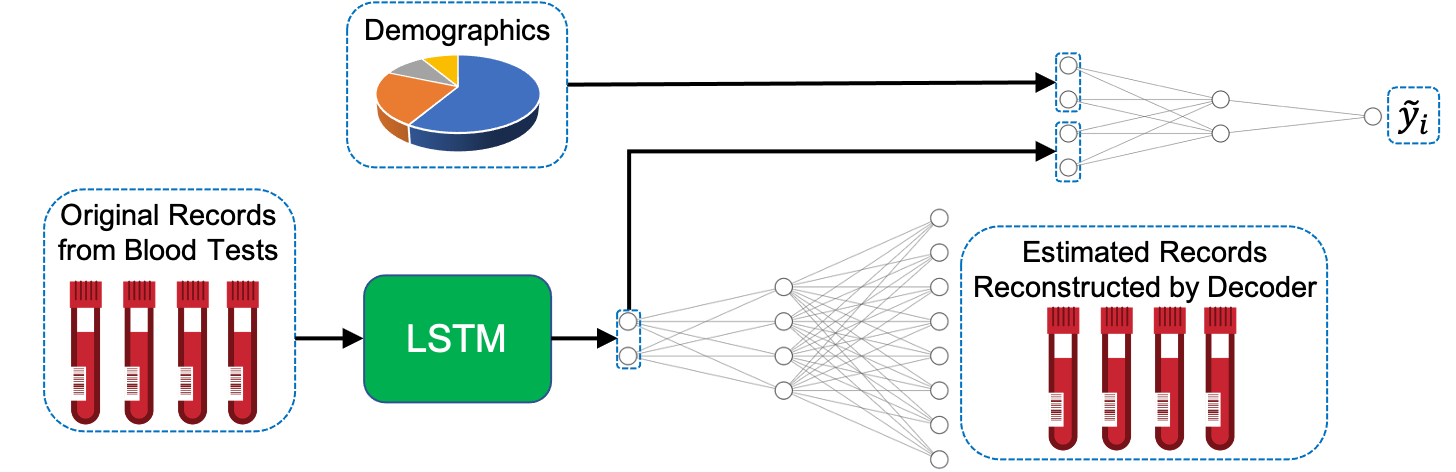
\includegraphics[width=1.0\textwidth]{figures/network-structure.png}
    \caption{The workflows of the enrichment learning task. The enriched representation at the bottleneck of the LSTM autoencoder is used to reconstruct the longitudinal records and predict the mortality.} \label{fig: LSTM and MLP}
\end{figure*}

\subsection{Dataset}
% Normalized, Min-max scaling. Time point to floating numbers, seconds after admission.
We obtain the blood sample records, demographic information, and associated mortality outcomes of 375 patients collected throughout their stay in Tongji hospital between 10th January and 24th February 2020 following the previous research~\cite{yan2020interpretable}. We discard 17 samples whose no time stamp is recorded. Among the remaining 358 samples, 192 patients survived (labeled as 1) and 166 patients died (labeled as 0). The order of samples is randomly shuffled to prevent the bias from the order. Each feature of dataset is normalized by min-max scaling to the range [0, 1]. 

\subsection{Notations}
In this paper, we denote a vector as a bold lower case letter, and matrix as a bold upper case letter. 
% For the arbitrary matrix $\mathbf{X}$, $\mathbf{x}^r$, $\mathbf{x}_c$, $x^r_c$ denotes the $r$-th row, $c$-th column, an element of $r$-th row and $c$-th column respectively. 
We use $i$ and $j$ to index $i$-th participant and $j$-th record respectively. We describe the records of $i$-th participant as $\mathcal{X}_i = \{\mathbf{x}_i^b, \mathbf{X}_i, \mathbf{M}_i, \mathbf{t}_i\}$ as follows:
\begin{itemize}
    \item $\mathbf{x}_i^b \in \Re^{D_b}$ is a vector of basic demographic information, such as age and gender.
    \item $\mathbf{X}_i = [\mathbf{x}_i^1; \mathbf{x}_i^2; \cdots; \mathbf{x}_i^{n_i}] \in \Re^{n_i \times D_l}$ are the longitudinal records collected from the blood tests across the $n_i$ time points.
    \item $\mathbf{M}_i = [\mathbf{m}_i^1; \mathbf{m}_i^2; \cdots; \mathbf{m}_i^{n_i}] \in \{1, 0\}^{n_i \times D_l}$ are the binary masks of observabilities of longitudinal records $\mathbf{X}_i$, where 1 and 0 indicates the observed and unobserved entry respectively.
    \item $\mathbf{t}_i = [t_i^1; t_i^2; \cdots; t_i^{n_i}] \in \Re^{n_i}$ are the time stamps of $n_i$ records.
\end{itemize}
The missing entries in $\mathbf{X}_i$ are initialized with the constant $-1$, and this value does not affect the result. The target label $\mathbf{y}_i \in \{0, 1\}$ is the mortality of $i$-th participant, which is provided in the training process if that participant is in training set, such that $i \in \Omega$.

\subsection{Encoder}
We leverage LSTM encoder $\phi_{E}: \Re^{n_i \times (2 D_l + 1)} \mapsto \Re^{d_z}$ to summarize the longitudinal records and learn the temporal relation between records. The time stamp of each record is crucial in learning the temporal relation between records (e.g. temporal locality), while the the missingness pattern of the entries may represent the participants' status. Thus we provide the concatenation of longitudinal records, masks, and time stamps, $[\mathbf{X}_i, \mathbf{M}_i, \mathbf{t}_i] = [\hat{\mathbf{x}}_i^1; \hat{\mathbf{x}}_i^2; \cdots; \hat{\mathbf{x}}_i^{n_i}] = \hat{\mathbf{X}}_i \in \Re^{n_i \times (2 D_l + 1)}$, as an input of LSTM encoder such that $\phi_{E}(\mathbf{X}_i, \mathbf{M}_i, \mathbf{t}_i;\ \theta_E) = \mathbf{z}_i$. Here, $\theta_E$ denotes the set of trainable parameters of LSTM.

For each time step ($1 \leq j \leq n_i$), the input record $\hat{\mathbf{x}}_i^j$ of $i$-th patient is processed by following the LSTM architecture~\cite{yu2019review}:
\begin{equation}
    \mathbf{k}^j_i = \sigma(\hat{\mathbf{x}}^j_i \mathbf{W}_{xk} + \mathbf{h}_i^{j-1} \mathbf{W}_{hk} + \mathbf{c}_i^{j-1} \mathbf{W}_{ck} + \mathbf{b}_k),
\end{equation}
\begin{equation}
    \mathbf{f}^j_i = \sigma(\hat{\mathbf{x}}^j_i \mathbf{W}_{xf} + \mathbf{h}^{j-1}_i \mathbf{W}_{hf} + \mathbf{c}^{j-1}_i \mathbf{W}_{cf} + \mathbf{b}_f),
\end{equation}
\begin{equation}
    \mathbf{c}^j_i = \mathbf{f}^j_i \odot \mathbf{c}^{j-1}_i + \mathbf{k}^j_i \odot \operatorname{tanh}(\hat{\mathbf{x}}_i^j \mathbf{W}_{xc} + \mathbf{h}^{j - 1}_i \mathbf{W}_{hc} + \mathbf{b}_c),
\end{equation}
\begin{equation}
    \mathbf{o}^j_i = \sigma(\hat{\mathbf{x}}_i^j \mathbf{W}_{xo} + \mathbf{h}^{j-1}_i \mathbf{W}_{ho} + \mathbf{c}^j_i \mathbf{W}_{co} + \mathbf{b}_o),
\end{equation}
\begin{equation}
    \mathbf{h}^j_i = \mathbf{o}^j_i \odot \operatorname{tanh}(\mathbf{c}^j_i),
\end{equation}
where $\sigma$ and tanh is the logistic sigmoid and hyperbolic tangent activation function respectively, and $\mathbf{k}^j_i$, $\mathbf{o}^j_i$, $\mathbf{f}^j_i$ are input, output, forget gate of $j$-th time step respectively. \{$\mathbf{W}_{xk}$, $\mathbf{W}_{hk}$, $\mathbf{W}_{ck}$, $\mathbf{W}_{xf}$, $\mathbf{W}_{hf}$, $\mathbf{W}_{cf}$, $\mathbf{W}_{xc}$, $\mathbf{W}_{hc}$, $\mathbf{W}_{xo}$, $\mathbf{W}_{ho}$, $\mathbf{W}_{co}$\} $\subset \mathbf{\theta}_E$ are trainable weight matrices and $\{\mathbf{b}_k, \mathbf{b}_f, \mathbf{b}_c, \mathbf{b}_o\} \subset \mathbf{\theta}_E$ are trainable bias vectors. $\mathbf{c}_i^j$ and $\mathbf{h}_i^j$ denote the cell state and hidden representation at $j$-th time step. The hidden representation $\mathbf{h}_i^{n_i}$ at the last time step $n_i$ is our enriched representation of the longitudinal records $\hat{\mathbf{X}}_i$, such that $\mathbf{h}_i^{n_i} = \mathbf{z}_i \in \Re^{d_z}$.
\begin{equation}
    \mathbf{h}_i^{n_i} = \mathbf{z}_i = \phi_E(\mathbf{X}_i, \mathbf{M}_i, \mathbf{t}_i; \mathbf{\theta}_E).
\end{equation}
Since the hidden representation at $j$-th time point aims to summarize the records from first time step to $j$-th time step, the LSTM cell needs to refer to the cell state $\mathbf{c}_i^j$ and reflect past records to $\mathbf{h}_i^j$. Since the cell state $\mathbf{c}_i^j$ is guided by the input gate $\mathbf{k}_i^j$ and forget gate $\mathbf{f}_i^j$, which control how much information came from previous step should be preserved, the cell state $\mathbf{c}_i^j$ enables the hidden representation $\mathbf{h}_i^j$ to learn long term dependencies. For example, LSTM encoder can capture the temporal trends of patient's status from the consecutive records.

% \subsubsection{Autoencoder}
% The encoder $\phi: \Re^{n_i \times (2 D_l + 1)} \mapsto \Re^{D_z}$ maps the input MTS in the high dimensional space into the latent representation in the lower dimensional space, such that $\phi_E(\mathbf{X}_i, \mathbf{M}_i, \mathbf{t}_i; \mathbf{\theta}_E) = \mathbf{z}_i \in \Re^{D_z}$. From the enriched representation $\mathbf{z}_i$, decoder $\phi_D: \Re^{D_z + 1} \mapsto \Re^{D_l}$ reconstructs the original record $\phi_D(\mathbf{z}_i ,t_i^j; \mathbf{\theta}_D) = \tilde{\mathbf{x}}_i^j \in \Re^{D_l}$, for each time point $t_i^j$ ($1 \leq j \leq n_i$). The predictor $\phi_P: \Re^{D_z + D_b} \mapsto [0, 1]$ generates the prediction $\phi_P(\mathbf{z}_i, \mathbf{x}_i^b; \mathbf{\theta}_P) = \tilde{y}_i$. $D_b, D_l, D_z$ denote the dimensionality of static, longitudinal, enriched biomarkers, and $\mathbf{\theta}_E, \mathbf{\theta}_D, \mathbf{\theta}_P$ denote the trainable parameters of encoder, decoder, predictor, respectively. 
% % Then we combine encoder, decoder, and predictor as a composite model, illustrated in Fig.~\ref{fig: autoencoder}.

% \subsection{Encoder}
% We leverage an LSTM encoder to compress MTS and extract long term dependencies in the temporal trend. 
% \subsubsection{Input}
% Because the time stamp of each record is crucial to learn the temporal trend and missingness pattern of the entries may represent the state of patient, we provide the concatenation of longitudinal records, masks, and time stamps $[\mathbf{X}_i, \mathbf{M}_i, \mathbf{t}_i] = \hat{\mathbf{X}}_i = [\hat{\mathbf{x}}_i^1; \hat{\mathbf{x}}_i^2; \cdots; \hat{\mathbf{x}}_i^{n_i}] \in \Re^{n_i \times (2 D_l + 1)}$ to the input layer of LSTM encoder. 
% The inputs of LSTM are $\hat{\mathbf{x}}_i^j$, $\mathbf{h}_{j - 1}$, $\mathbf{c}_{j - 1}$ and outputs are $\mathbf{h}_{j}$ and $\mathbf{c}_{j}$, where $\mathbf{h}_{j}$ is the hidden representation of records and $\mathbf{c}_{j}$ is the cell state of LSTM cell at $j$-th time step. 

% \subsubsection{Output}
% For each time step ($1 \leq j \leq n_i$), the input record $\hat{\mathbf{x}}_i^j$ of $i$-th patient is processed by following the LSTM architecture~\cite{yu2019review}:
% % The hidden representation $\mathbf{h}_j$ should compress the longitudinal records from first time step to $j$-th time step to accurately reconstruct the records, and the final hidden representation $\mathbf{h}_{n_i} = \mathbf{z}_i$ is the encoded representation of longitudinal records.
% \begin{equation}
%     \mathbf{k}^j_i = \sigma(\hat{\mathbf{x}}^j_i \mathbf{W}_{xk} + \mathbf{h}_i^{j-1} \mathbf{W}_{hk} + \mathbf{c}_i^{j-1} \mathbf{W}_{ck} + \mathbf{b}_k),
% \end{equation}
% \begin{equation}
%     \mathbf{f}^j_i = \sigma(\hat{\mathbf{x}}^j_i \mathbf{W}_{xf} + \mathbf{h}^{j-1}_i \mathbf{W}_{hf} + \mathbf{c}^{j-1}_i \mathbf{W}_{cf} + \mathbf{b}_f),
% \end{equation}
% \begin{equation}
%     \mathbf{c}^j_i = \mathbf{f}^j_i \odot \mathbf{c}^{j-1}_i + \mathbf{k}^j_i \odot \operatorname{tanh}(\hat{\mathbf{x}}_i^j \mathbf{W}_{xc} + \mathbf{h}^{j - 1}_i \mathbf{W}_{hc} + \mathbf{b}_c),
% \end{equation}
% \begin{equation}
%     \mathbf{o}^j_i = \sigma(\hat{\mathbf{x}}_i^j \mathbf{W}_{xo} + \mathbf{h}^{j-1}_i \mathbf{W}_{ho} + \mathbf{c}^j_i \mathbf{W}_{co} + \mathbf{b}_o),
% \end{equation}
% \begin{equation}
%     \mathbf{h}^j_i = \mathbf{o}^j_i \odot \operatorname{tanh}(\mathbf{c}^j_i),
% \end{equation}
% where $\sigma$ is logistic sigmoid activation function and $\mathbf{k}^j_i$, $\mathbf{o}^j_i$, $\mathbf{f}^j_i$ are input, output, forget gate of $j$-th time step respectively. \{$\mathbf{W}_{xk}$, $\mathbf{W}_{hk}$, $\mathbf{W}_{ck}$, $\mathbf{W}_{xf}$, $\mathbf{W}_{hf}$, $\mathbf{W}_{cf}$, $\mathbf{W}_{xc}$, $\mathbf{W}_{hc}$, $\mathbf{W}_{xo}$, $\mathbf{W}_{ho}$, $\mathbf{W}_{co}$\} $\subset \mathbf{\theta}_{E}$ are trainable weights matrix and $\{\mathbf{b}_k, \mathbf{b}_f, \mathbf{b}_c, \mathbf{b}_o\} \subset \mathbf{\theta}_{E}$ are trainable bias vectors. $\mathbf{c}_i^j$ and $\mathbf{h}_i^j$ denote the cell state and hidden representation. 

% In order decoder and predictor to reconstruct the original record and predict the target label accurately, the enriched representation should contain enough information for reconstruction and prediction, such as temporal trend of input sequence. The goal of encoder at $j$-th time pont is to generate the hidden representation $\mathbf{h}_i^j$ summarizing the records from first time step to $j$-th time step, therefore the LSTM cell refers to the cell state $\mathbf{c}_i^j$ and reflect the past records to $\mathbf{h}_i^j$. Since the cell state $\mathbf{c}_i^j$ is guided by the input gate $\mathbf{k}_i^j$ and forget gate $\mathbf{f}_i^j$ which control how much information came from previous step should be preserved, the cell state $\mathbf{c}_i^j$ enables the hidden representation $\mathbf{h}_i^j$ to learn the long term dependencies. For example, if the differences in the records and time intervals between the time points of recent 10 consecutive records are small, the hidden representation of 10 time steps before can be preserved.
% % and  and  Because input gate $\mathbf{k}_i^j$ and forget gate $\mathbf{f}_i^j$ control how much we keep the information came from previous step, therefore LSTM is able to convey the most useful inf
% The hidden representation $\mathbf{h}_i^{n_i}$ at the most recent time point is the enriched representation $\mathbf{z}_i$ of whole longitudinal records of $i$-th patent:
% % Then the enriched representation $\mathbf{z}_i$ is given to the decoder and predictor.
% \begin{equation}
%     \mathbf{h}_i^{n_i} = \mathbf{z}_i = \phi_E(\mathbf{X}_i, \mathbf{M}_i, \mathbf{t}_i; \mathbf{\theta}_E).
% \end{equation}

\subsection{Decoder and Predictor}
From the enriched representation $\mathbf{z}_i$ of longitudinal records, the decoder reconstruct the original record, and predictor predicts the target label.
The decoder and predictor both are the multilayer perceptron (MLP), instead of LSTM. A previous study~\cite{srivastava2015unsupervised} that attempted to enrich longitudinal records with a recurrent neural network (RNN)~\cite{medsker2001recurrent}, did so by using RNNs for both the encoder and decoder, where the output (reconstructed record) of the decoder at each time step depends on the output at the previous time step. However, since no additional information is provided to the decoder other than a learned representation that is no longer longitudinal, there should not be dependency between the outputs of the decoder. Because the enriched representation $\mathbf{z}_i$ summarizes \emph{whole} longitudinal records, the decoder $\phi_D:\Re^{d_z + 1} \mapsto \Re^{D_l}$ should be able to reconstruct the $j$-th record $\mathbf{x}_i^j$ given time stamp $t_i^j$ without any additional information, such that $\phi_D(\mathbf{z}_i, t^j_i;\ \theta_D) = \tilde{\mathbf{x}}_i^j \approx \mathbf{x}_i^j$, where $\theta_D$ is a set of weight matrices and bias vectors of the decoder. This autoencoder architecture, to the best of our knowledge, has not yet been proposed. 

MLP consists of the consecutive hidden layers as follows:
\begin{equation}
    \mathbf{h}_k = \sigma(\mathbf{W}_k\mathbf{h}_{k-1} + \mathbf{b}_k),
\end{equation}
where $\mathbf{h}_k$ is the output of $k$-th hidden layer, and $\sigma$ is the activation function, and $\mathbf{W}_k$, $\mathbf{b}_k$ are the trainable weights matrix and bias vector of $k$-th hidden layer. The output is earned by forwarding the input vector $\mathbf{h}_0$ to the last hidden layer. To recover the original record at the specific time point, the decoder needs to know that time point. Thus the input vector of decoder is the concatenation of enriched representation $\mathbf{z}_i$ and time stamp $t^j_i$, which is $[\mathbf{z}_i, t_i^j] \in \Re^{d_z + 1}$. For predictor, the demographic information such as age may be crucial to predict target label. Therefore we provide the demographic information to the predictor with the enriched representation, which is $[\mathbf{z}_i, \mathbf{x}_i^b] \in \Re^{d_z + D_b}$. By forwarding each input of decoder and predictor to their own MLP, we earn the reconstructed record $\tilde{\mathbf{x}}_i^j$ and prediction $\tilde{y}_i$ on target label:
\begin{equation}
    \phi_D(\mathbf{z}_i, t_i^j; \mathbf{\theta}_D) = \tilde{\mathbf{x}}_i^j,
\end{equation}
\begin{equation}
    \phi_P(\mathbf{z}_i, \mathbf{x}_i^b; \mathbf{\theta}_P) = \tilde{\mathbf{y}}_i,
\end{equation}
and we have the stack of reconstructed records of $i$-th patient:
\begin{equation}
    \tilde{\mathbf{X}}_i = [\tilde{\mathbf{x}}_i^1; \tilde{\mathbf{x}}_i^2; \cdots; \tilde{\mathbf{x}}_i^{n_i}].
\end{equation}
\begin{figure*}[t]
    \centering
    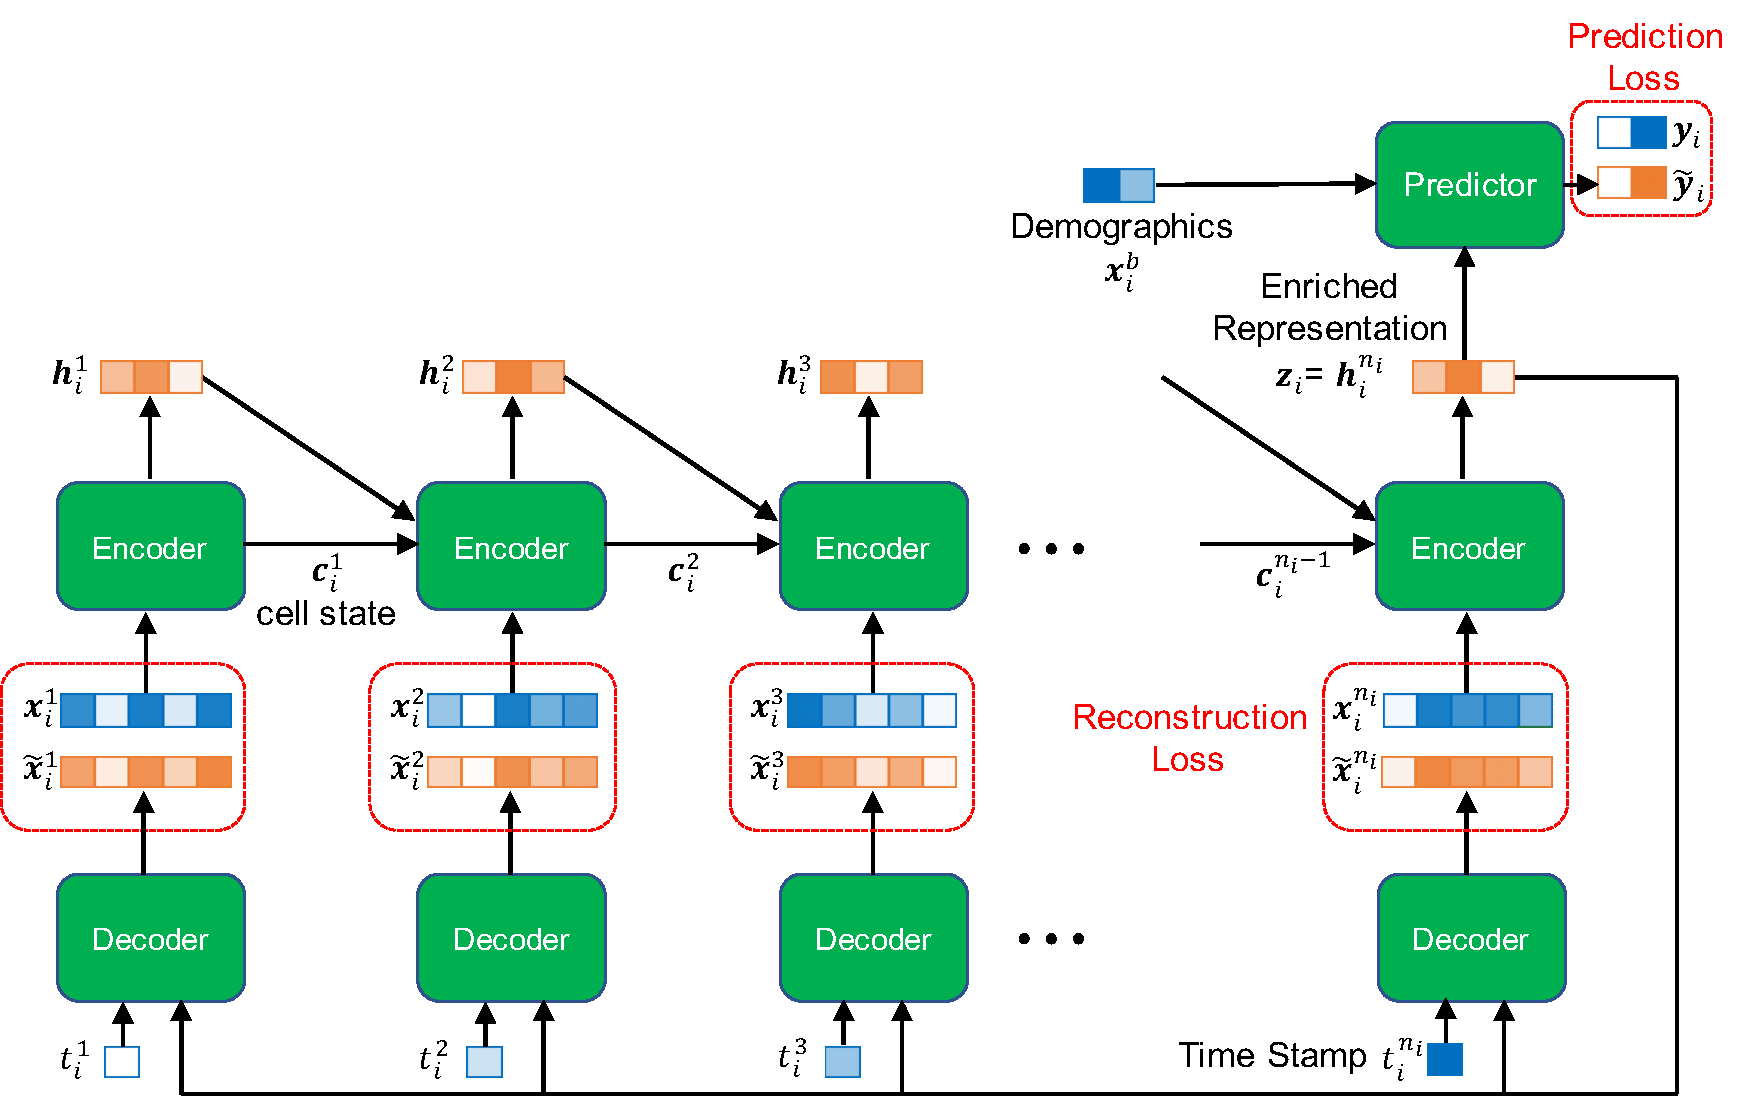
\includegraphics[width=0.9\textwidth]{figures/autoencoder.pdf}
    \caption{An illustration for the loss functions. The encoder consists of LSTM cell, which processes input record $\mathbf{x}_i^j$, and then generates the hidden representation $\mathbf{h}_i^j$ while conveying the cell state $\mathbf{c}_i^j$ to the next step. The enriched representation of the whole time series is defined as the hidden representation $\mathbf{h}_i^{n_i}$ at the last step.} \label{fig: autoencoder}
\end{figure*}
% \begin{equation}
%     \mathbf{\tilde{x}}_i^j = \sigma(\mathbf{W}_3 \sigma(\mathbf{W}_2 \sigma(\mathbf{W}_1 [\mathbf{z}_i, t_i^j] + \mathbf{b}_1) + \mathbf{b}_2) + \mathbf{b}_3) \sigma(\mathbf{W}_k\mathbf{h}_{k-1} + \mathbf{b}_k)
% \end{equation}
% In other words, the decoder should be able to reconstruct the original record with enriched vectorial representation $\mathbf{z}_i$ and time stamp $t_i^j$ if $\mathbf{z}_i$ successfully summarizes the records of all time steps. 

\subsection{Loss Functions}
AE is asked to accomplish the two tasks - reconstructing original records and predicting target label by minimizing:
\begin{equation}\label{eq: objective}
    \min_{\theta_E, \theta_D, \theta_P} \mathcal{L}_{total} = \min_{\theta_E, \theta_D, \theta_P}(\gamma_1\mathcal{L}_{reconstruct} + \gamma_2\mathcal{L}_{predict}),
\end{equation}
where $\gamma_1$ and $\gamma_2$ are the hyperparameters to adjust the impact of each loss.
The reconstruction loss is defined as the scaled Mean Squared Error (MSE):
\begin{equation}
    \mathcal{L}_{reconstruct} = \frac{\left\| (\tilde{\mathbf{X}}_i - \mathbf{X}_i) \odot \mathbf{M}_i \right\|_F^2}{|\mathbf{M}_i|},
\end{equation}
where squared Frobenious norm $\| \cdot \|_F^2$ is defined as the summation of all the entries squared.

The the prediction loss is defined respect to the labeled $i \in \Omega$ and unlabeled $i \not\in \Omega$ data separately:
\begin{equation}
    \mathcal{L}_{predict} = \left\{\begin{array}{lr}
        \| \tilde{y}_i - y_i \|_F^2, & \text{for } i \in \Omega\\
        0, & \text{for } i \not\in \Omega
    \end{array}\right\}.
\end{equation}
The high capacity unsupervised AE may suffer from the tendency to learn the trivial identity mapping and memorize the input~\cite{srivastava2015unsupervised}. The addition of prediction loss can prevent this memorization problem, because the memorization is not useful to predict the target label.

%Here the encoder LSTM is asked to come up with a state from which we can both predict the next few frames as well as reconstruct the input.
% This composite model tries to overcome the shortcomings that each model suffers on its own. A high-capacity autoencoder would suffer from the tendency to learn trivial representations that just memorize the inputs. However, this memorization is not useful at all for predicting the future. Therefore, the composite model cannot just memorize information.

% $L_{pred}$ is 0 when test set.
% Structure of LSTM, and if decoder is LSTM, then which state should be passed?
% Image for input (static + dynamic concatenation) and output (RE\_DATE is concatenated), and prediction target.
% LSTM unit explanation with maybe Figure. Concatenate static features because they are helpful to learn enrichment.
% Figure : Balance, reconstruction error vs prediction error.
% Why decoder is not RNN? Think of what is input for encoder and decoder. Because there is no information is additionally provided, current prediction depends on previous prediction does not make sense. The enriched representation is the fixed-length vector which is not longitudinal records anymore.